\centerline{
\begin{tikzpicture}
%\end{axis}
\begin{axis}[
    width=1\textwidth,
    height=.22\textheight,
    ymin=0,ymax=17,
   % xmin=0,xmax=21,
    xtick={0,...,15},
    xticklabels={},
    %x tick label style={color=white},
	ylabel={Iterations},
	axis y line*=left,
	enlargelimits=0.05,
	legend style={at={(0.5,-0.4)},
	anchor=north,legend columns=-1},
	ylabel near ticks,
	ybar,
	%ymajorgrids=true,
	%xmajorgrids=false,
    grid style=dashed
]
%\addlegendimage{blue, mark=*}
%\addlegendimage{only marks, orange!80, mark=square*}
%\addlegendimage{only marks, purple!70, mark=square*}
%\legend{Accuracy, Train time, Test time}
\addplot[color=orange!80,fill=orange!80]
	coordinates {
	(0,6) (2,15) (3,5) (4,3) (5,2) (7,7) (8,15) (9,15) (10,15) (12,9) (13,15) (14,15) (15,15)
    };
\end{axis}
\begin{semilogyaxis}[
%\begin{axis}[
    title={Iterations and accuracy of different sub-sampeling settings},
    width=\textwidth,
    height=.22\textheight,
    ymin=0.0001, ymax=1,
    %xmin=0,xmax=21,
	xtick={0,...,15},
	xticklabels={
		%linear,poly:d=2,poly:d=3,poly:d=4,poly:d=5,poly:d=6,poly:d=7,poly:d=8,poly:d=9,rbf:$\gamma$=0.0,rbf:$\gamma$=0.1,rbf:$\gamma$=0.2,rbf:$\gamma$=0.3,rbf:$\gamma$=0.4,rbf:$\gamma$=0.5,rbf:$\gamma$=0.6,rbf:$\gamma$=0.7,rbf:$\gamma$=0.8,rbf:$\gamma$=0.9,rbf:$\gamma$=1.0,
		all,$\,$,$sample_{2}$,$sample_{17}$,$sample_{47}$,$sample_{91}$,$\,$,$rand1_{0.8}$,$rand1_{0.5}$,$rand1_{0.1}$,$rand1_{0.01}$,$\,$,$randi_{0.8}$,$randi_{0.5}$,$randi_{0.1}$,$randi_{0.01}$,
	},
	x tick label style={rotate=30, anchor=north east, inner sep=0mm},
	%xlabel={\hspace{1cm}${\underbrace{\text{\hspace{5cm}}}\atop\text{polynomial}}$\hspace{0.4cm}${\underbrace{\text{\hspace{7cm}}}\atop\text{rbf}}$},
	%xlabel style={at={(0.5,-0.03)}},
	ylabel=Mean Squared Error,
	axis y line*=right,
	enlargelimits=0.05,
	legend style={at={(0.5,-0.4)},
	anchor=north,legend columns=-1},
	%ybar stacked,
	ylabel near ticks
]
\addplot[mark=*,blue,jump mark mid]
	coordinates {
	(-1,1000) (0,0.0018) (1,1000) (2,0.0027) (3,0.0007) (4,0.0006) (5,0.0006) (6,1000) (7,0.0019) (8,0.0025) (9,0.0125) (10,0.1677) (11,1000) (12,0.0017) (13,0.0031) (14,0.0249) (15,0.485) (17,1000)
    };
\end{semilogyaxis}
\end{tikzpicture}
}